\subsection{Rock Salt Samples}
\label{subsec:salt}
\Authors{Mathias Nest, Dirk Naumann (IfG)}

\subsubsection{The Springen in-situ laboratory}
\label{sec:springen}

The large-scale test site Merkers benefits from the unique mining situation in the bedded salt mass of the Werra salt formation (z1, Zechstein sequence) where two potash seams were mined in a room-and-pillar system at 275 m (1st floor, potash seam ''Hessen'', z1KH) and 360 m (2nd floor, potash seam ''Thüringen'', z1KTh) depth, respectively. Fig. \ref{fig:springenlab} shows the preparation of an experiment on the 2nd seam. The evaporite rocks of the Zechstein formation were laid down during the Permian period around 250 million years ago. The intact mineral deposit was locally disturbed between 14 and 25 million years ago by tertiary volcanism, leading to the mutation of some potash salts to sylvinite, and the creation of pockets of CO$_2$ under high pressure.

\begin{figure}[ht!]
\centering
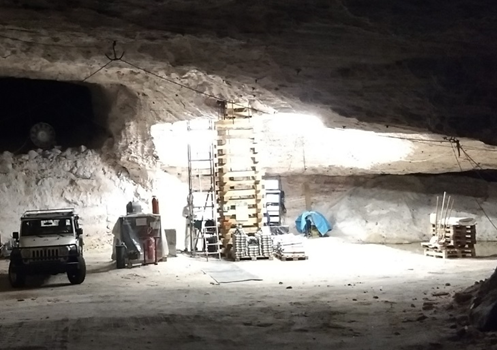
\includegraphics[width=0.85\textwidth]{figures/springen2ndseam.png}
\caption{Preparation of experiments on the second seam.}
\label{fig:springenlab}
\end{figure}

The pressurized tests are conducted between the two potash seams in the very homogeneous Middle Werra rocksalt (z1Na). It consists mostly of very pure halite layers intersected by thin anhydrite lines or bands of rocksalt with finely distributed anhydrite accessories indicating the sedimentary bedding. 

Because the test results depend mainly on the acting stress field, i.e. the minimal stress distribution in the rock mass around the test area, it has been measured and  characterized by hydro-frac measurements, and is thus well-known. The minimal stresses in the contour increase with progressive distances from the underground openings until reaching a constant value in a depth of around 15 m. The measured value of an undisturbed stress state of around 8 MPa corresponds fairly well to calculated lithostatic stresses of 7.8 to 8.8 MPa. 

The main facility is a large borehole of nearly vertical 60 m height and 1.3 m diameter. It was drilled upwards from the second floor, ending about 20 m beneath the first floor. For access to the later sealed volume an 85 mm pilot hole has been drilled from the upper floor. The borehole was closed by a 20 m high MgO-concrete plug. 

For monitoring of micro-seismic events, e.g. due to creation of an excavated damage zone around underground openings or fluid flow driven damage, a highly sensitive AE-network was installed in observation boreholes, which were drilled parallel to the main borehole. This network has constantly been updated and extended over the past years. Signals of magnitude M $<$ -4 can be detected in a frequency range from 1 kHz to 200 kHz. This corresponds to intergranular microcracking on grain boundaries on a millimeter- to centimeter-scale. 

\subsubsection{Rock salt laboratory}

The following conditions and equipment are available in the IfG labs for rock mechanical laboratory investigations:

\begin{list}{-}{\leftmargin=1em \itemindent=0em \itemsep=0.1em}
\item Climate-controlled rooms for storage of specimens at conditions which correspond to those present in situ
\item Laboratory for mineral-petrographic examinations, density and moisture determination, ultra-sound measurements and 
photographic documentation
\item Workshop for the preparation of specimens in high precision according to testing requirements (rock saws, lathes etc.)
\item Test laboratory containing various servo-controlled hydraulic testing machines for conducting investigations on 
rock mechanics in accordance with the up-to-date state of research and development (see Figure \ref{fig:ifglabph1}).
\end{list} 

\begin{figure}[!ht]
\centering
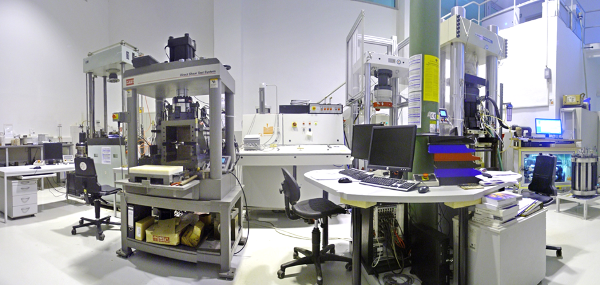
\includegraphics[width=1\textwidth]{./figures/ifg-lab-photo1-v2.png}
\caption{View inside the rock mechanical lab with various servo-controlled hydraulic testing machines.}
\label{fig:ifglabph1}
\end{figure}

It has to be mentioned that some of the applied IfG test procedures have been developed for the requirements of the specific IfG-material laws. 
But generally they are in accordance to ASTM and ISRM standards resp. equivalent descriptions, e.g.:

\begin{list}{-}{\leftmargin=1em \itemindent=0em \itemsep=0.1em}
\item ASTM D 4543-85 Standard Practice for Preparing Rock Core Specimens and Determining Dimensional and Shape Tolerances
\item ASTM D 2845-05 Standard Test Method for Laboratory Determination of Pulse Velocities and Ultrasonic Elastic Constants of Rock
\item ASTM D 2664-86 Standard Test for Triaxial Compressive Strength of Un\-drained Rock Core Specimens without Pore Pressure Measurements 
\item DGEG (1979):   Empfehlung Nr. 2 des AK 19 der DGEG (Dreiaxiale Druckversuche).
\item ASTM D4406-04 Standard Test Method for Creep of Cylindrical Rock Core Specimens in Triaxial Compression
\item ASTM D7070-04 Standard Test Method for Creep of Rock Core Under Constant Stress and Temperature
\item ISRM: Suggested Methods for Determining o the Uniaxial Compressive Strength and Deformability of Rock Materials
\item ISRM: Suggested Methods : Part 2 : 2007 - Unconfined Compressive Strength with Young's Modulus and Poisson's Ratio
\item ISRM: - Suggested Methods : Part 2 : Received 1983 - Strength of Rock Material in Triaxial Compression
\end{list}

\subsubsection{Sample characterization and pre-investigation}

Several preliminary investigations are usually done before lab testing. After preparing the cylindric samples (cutting with a rock saw and smoothing the samples with a lathe) in the IfG labs, their density is determined by measuring the geometrical dimensions and the mass. Concerning the quality of these parameters an accuracy in length determination is $<$ 0.01 mm, those in mass determination is $<$ 0.01 g. 

Additionally, ultrasonic investigations are carried out to check integrity, homogeneity and isotropy of the samples. The ultrasonic pulse measurement system used for transmission of the rock specimens consists of two transducer sets for P-waves and S-waves and a receiver system for generating and evaluating the ultrasonic signals. The specimen is placed in physical contact between two piezoelectric transducers, one acts as a driver and the other one acts as a receiver. The transit time of the mechanical pulse to pass through the specimen is used to determine elastic wave velocity.

For samples where both P- and S-waves were measured in axial sample direction the elastic constants are obtained from density ($\rho$) and the ultrasonic velocities ($v_p$, $v_s$) using the following expressions derived from the theory of elasticity for homogeneous, isotropic solids:

\begin{equation}
\label{eq:YoungsModulus_Ultrasonic}
E_{dyn} = \frac{\rho v_s^2(3v_p^2-4v_s^2)}{v_p^2-v_s^2} 
\end{equation}
\begin{equation}
\label{eq:PoissonsRatio_Ultrasonic}
\nu_{dyn} = \frac{v_p^2-2v_s^2}{2(v_p^2-v_s^2)}
\end{equation}

Dynamic elastic parameters of the various rock portions determined on the base of sonic wave velocity at room temperature are in a wide range representing typical values for the various materials as known from other locations. 

